\begin{frame}[fragile]{Tutorial: n-site states with MPS}

\begin{columns}

\begin{column}{5.5cm}

\begin{onlyenv}<1->
\begin{lstlisting}[language=JuliaLocal, style=julia, mathescape, basicstyle=\small]
$\psi_0$ = MPS(i, "Z+")
nlayers = 6
function F($\theta$)
  $\psi_\theta$ = apply(U($\theta$, i; nlayers), $\psi_0$)
  return -abs(inner($\psi$', $\psi_\theta$))^2
end

$\theta_0$ = zeros(nlayers * n)
$\theta$ = minimize(F, $\partial$F, $\theta_0$;
      nsteps=20, $\gamma$=0.1)
\end{lstlisting}
\end{onlyenv}

\begin{onlyenv}<3->
\begin{lstlisting}[language=JuliaLocal, style=julia, mathescape, basicstyle=\small]
maxlinkdim($\psi_0$)
maxlinkdim($\psi_\theta$)
F($\theta_0$), norm($\partial$F($\theta_0$))
F($\theta$), norm($\partial$F($\theta$))
\end{lstlisting}
\end{onlyenv}

\end{column}

\begin{column}{4.5cm}

\begin{onlyenv}<1-1>

\begin{lstlisting}[style=julia, numbers=none, mathescape, basicstyle=\small]
# |0$\rangle$ = |Z+Z+…Z+$\rangle$

# Minimize over $\theta$:
# F($\theta$) = -|$\langle\psi$|U($\theta$)|0$\rangle$|$^2$
#        = -|$\langle\psi$|$\theta\rangle$|$\^2$




 \end{lstlisting}

\end{onlyenv}

\begin{onlyenv}<2->
\vspace*{0.0cm}
\begin{center}
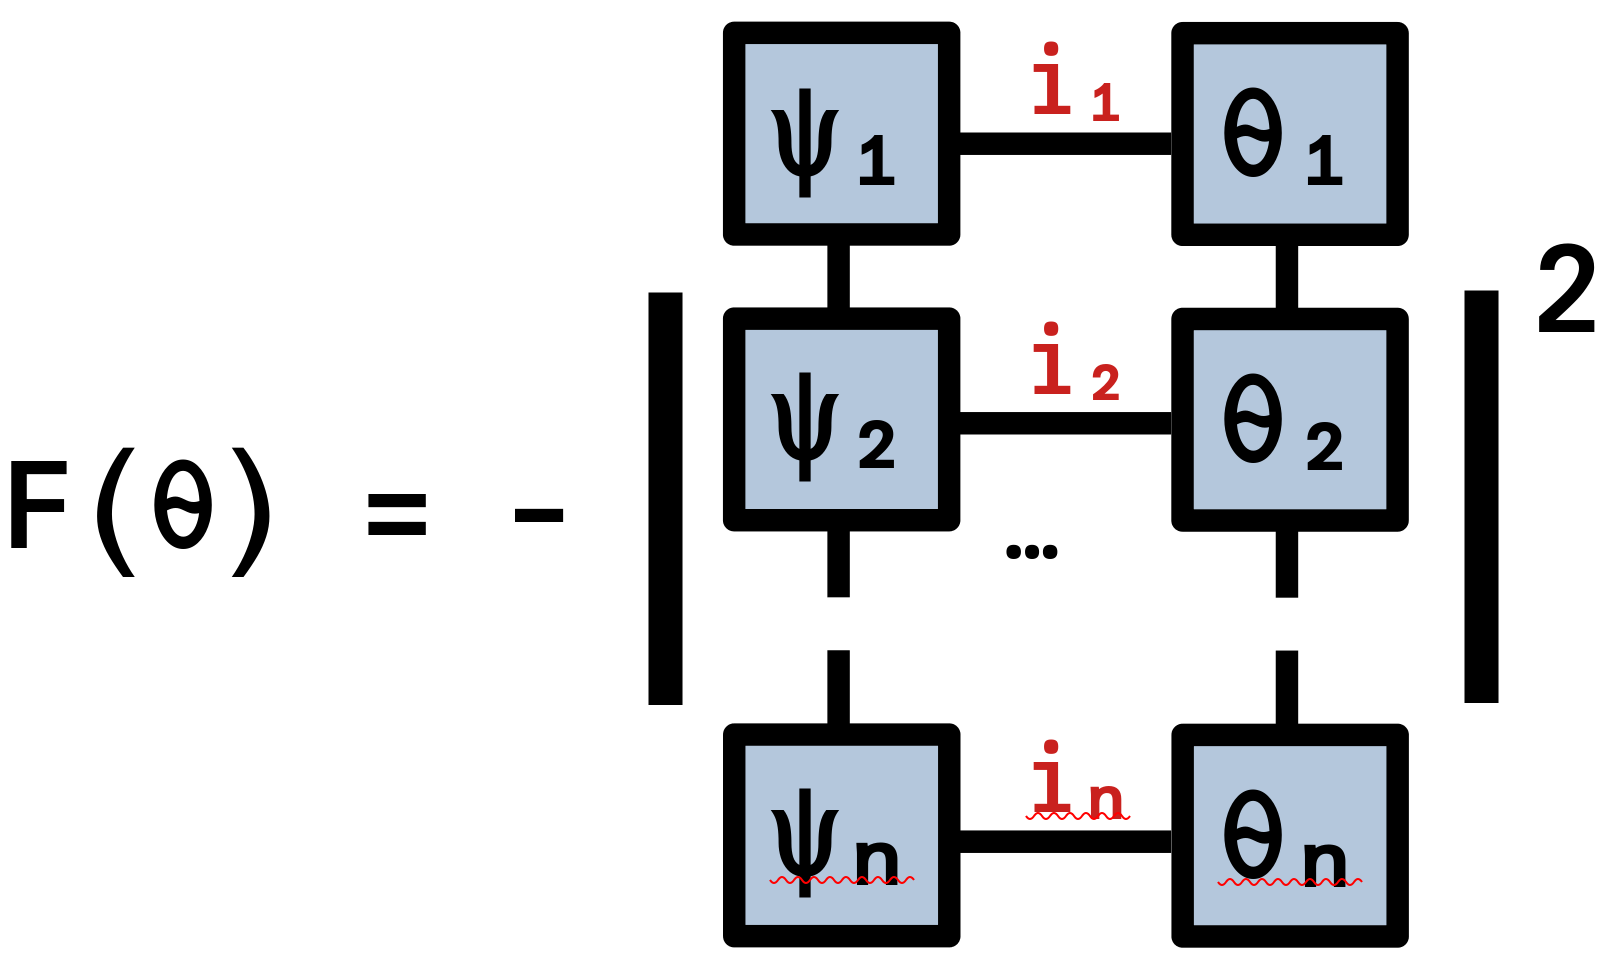
\includegraphics[width=\textwidth]{
  slides/assets/psin_thetan.png
} \\
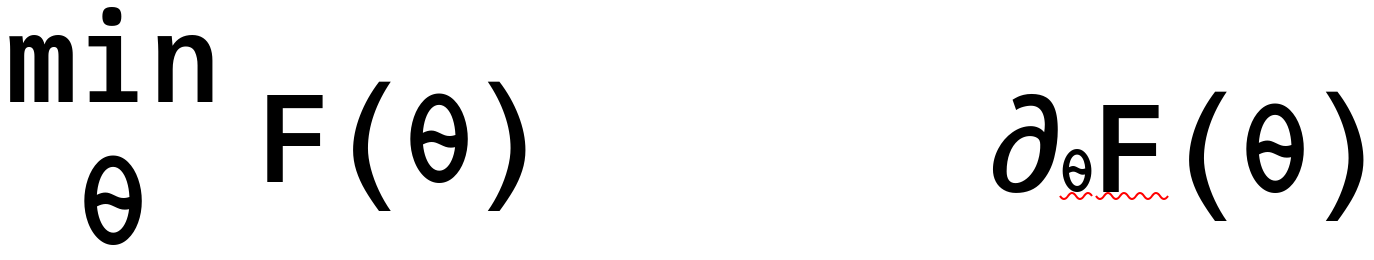
\includegraphics[width=\textwidth]{
  slides/assets/min_grad_F_theta.png
}
\end{center}
\vspace*{0.0cm}
\end{onlyenv}

\begin{onlyenv}<3->

\begin{lstlisting}[style=julia, numbers=none, mathescape, basicstyle=\small]
# 1 (product state)
# 2 (entangled state)
# (-0.556066, 0.895717)
# (-0.995230, 0.048939)
\end{lstlisting}

\end{onlyenv}

\end{column}

\end{columns}

\end{frame}
